As mentioned in ~\ref{sec: motivation}, a python tool is developed for this work. This chapter highlights its structure and elaborates on the details of implementation. Besides, several optimization strategies are discussed for the improvement of performance and memory usage.

\section{Why python?}

There are mainly two reasons for choosing Python over other compiled languages:

\begin{itemize}
    \item \textbf{Rapid Prototyping}: The fact that Python supports high-level language features makes it simpler to write code and to focus on readability and maintainability. This facilitates rapid prototyping in the scope of this thesis.
    \item \textbf{Rich Libraries Support}: Python has rich libraries support, including file I/O, parsing ELF file, parsing command line options, and matching patterns with regular expressions. As described more in the following sections, all of these libraries are helpful.
\end{itemize}

\section{Workflow}

Fig~\ref{fig:analyzer_structure} illustrates its structure. An \texttt{Analyzer} object instance takes an ELF file and its ETISS-generated instruction trace as inputs. The \texttt{Analyzer} internals (1) extract information from ELF file, (2) construct dynamic basic blocks, (3) aggregate callgrind inclusive costs, and (4) convert to callgrind output format file. 

\medskip
\dirtree{%
.1 TraceAnalysis/.
.2 main.py.
.2 lib/.
.3 \_\_init\_\_.py.
.3 analyzer.py.
.3 basicBlock.py.
}
\medskip

\subsection{Key Python Objects}

\lstset{
  language=Python,
  basicstyle=\footnotesize\ttfamily,
  breaklines=true,
  frame=single,
  keywordstyle=\color{blue},
  stringstyle=\color{red},
  commentstyle=\color{blue},
  showstringspaces=false,
  captionpos=b
}

\subsubsection{\texttt{Analyzer}}
\texttt{Analyzer} class is defined in \texttt{lib/analyzer.py}. It is the main class object that takes parameters from command line and performs core functionalities. Four parameters are taken from command line, namely \texttt{elf\_file\_path}, \texttt{trace\_file\_path}, \texttt{dump\_pc}, and \texttt{dump\_pos}. The two latter parameters specify desirable callgrind output format, which will be discussed in Section \ref{subsec:converter}. Besides, the method \texttt{run} executes internal methods \texttt{\_extract\_ELF\_information}, \texttt{\_build\_basicblocks}, and \texttt{\_callgrind\_output\_format\_converter} consecutively, which will be discussed in the following sections.

\begin{center}
\begin{minipage}{\textwidth}
\lstset{caption={\texttt{Analyzer} class object}}
\begin{lstlisting}
class Analyzer(object):
    def __init__(self, elf_file_path: str, trace_file_path: str, dump_pc: bool, dump_pos: bool):
    self.elf_file_path = elf_file_path
    self.trace_file_path = trace_file_path
    self.dump_pc = dump_pc
    self.dump_pos = dump_pos

    def run(self, callgrind_output_file_path: str):
        print("=====Extract ELF Information=====")
        self._extract_ELF_information()
        
        print("=====Building Basicblocks=====")
        self._build_basicblocks()

        print("=====Converting To Callgrind Output Format")
        self._callgrind_output_format_converter(callgrind_output_file_path)
        print("=====Conversion Done=====")

    
\end{lstlisting}
\end{minipage}
\end{center}

\subsubsection{\texttt{BasicBlock}}

\texttt{BasicBlock} class is defined in \texttt{lib/basicBlock.py}. A \texttt{BasicBlock} instance contains variables \texttt{first\_pc}, \texttt{last\_pc}, \texttt{last\_instr}, and \texttt{func}. Section \ref{subsec:bb_construction} and section \ref{subsec:basicblock_optimization} will discussed its usage and possibility for optimization. 

\begin{center}
\begin{minipage}{\textwidth}
\lstset{caption={\texttt{BasicBlock} class object}}
\begin{lstlisting}
class BasicBlock(object):
    def __init__(self, first_pc: int, last_pc: int, last_instr: str, func: str):
        self.first_pc = first_pc
        self.last_pc = last_pc
        self.func = func
        self.last_instr = last_instr
    
\end{lstlisting}
\end{minipage}
\end{center}


\begin{figure}
    \centering
    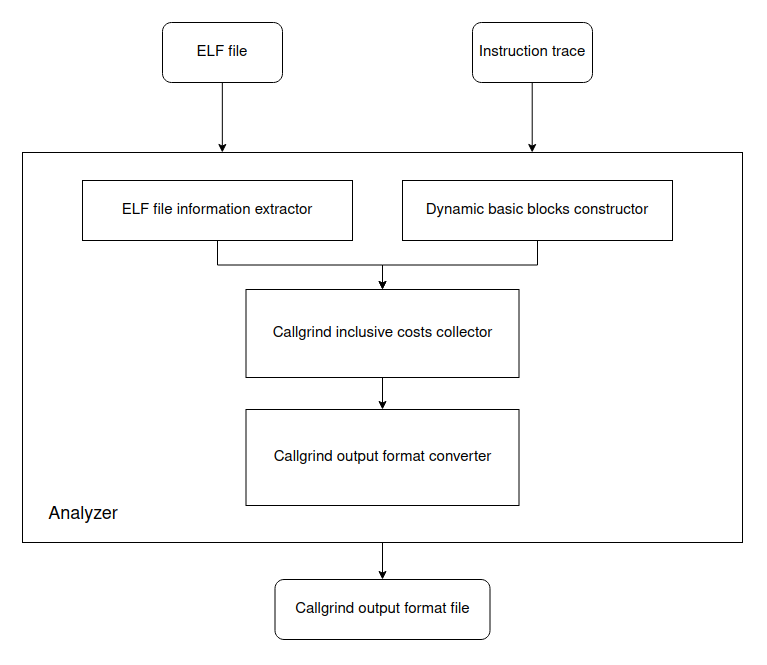
\includegraphics[width=\linewidth]{figures/Analyzer_structure.png}
    \caption{Workflow}
    \label{fig:analyzer_structure}
\end{figure}

\subsection{ELF File Information Extraction} 
\label{subsec:elf_info_extraction}

The first thing happens inside \texttt{Analyzer} internals is extracting information from ELF. Specifically, we need (1) the mapping between static program and dynamic traces, (2) the mapping between source files and functions, and (3) the mapping between program counters and source lines.

\subsubsection{Static Program - Dynamic Traces Mapping}
\label{subsubsec:pc_func_mapping}

Static program and dynamic traces are high-level terms. Concretely, we need the mapping between function and program counter range. In python, there is a well-developed library called \textit{pyelftools}, which is for parsing and analyzing ELF and DWARF debug information.~\cite{pyelftools_manual} The code in listing~\ref{code:func_pc_mapping} uses \textit{pyelftools} to construct mapping.

With the mapping available, utility function in Alg.\ref{alg:query_func_name} queries the function that a program counter of interest belongs to, which is extensively used in ~\ref{subsec:bb_construction} and in ~\ref{subsec:converter}.

\medskip
\begin{algorithm}
\caption{Utility function: function name query}
\label{alg:query_func_name}
\begin{algorithmic}
\REQUIRE $pc$, program counter
\REQUIRE $mapping$, mapping between function and program counter range
\FOR{$function$ in $mapping$}
    \IF{$function\_start\_pc \leq pc \leq function\_end\_pc$}
        \RETURN $function\_name$
    \ELSE
        \RETURN $None$
    \ENDIF
\ENDFOR
\end{algorithmic}
\end{algorithm}

\subsubsection{Source Files - Functions Mapping}
Callgrind output format conversion, which will be discussed in sec \ref{subsec:converter}, requires the mapping between source files and functions. The code in listing \ref{code:srcFile_func_mapping} extract the mapping with the help of \textit{pyelftools} library from DWARF core section. Also, a helper function for getting file name is shown in listing \ref{code:helper_function}.

\medskip

\begin{center}
\begin{minipage}[t]{\textwidth}
\lstset{caption={Function that extracts static program - dynamic traces mapping}, label=code:func_pc_mapping}
\begin{lstlisting}[language=Python]
from elftools.elf.elffile import ELFFile

## Assume elf_file_path is given
pc_to_func_mapping = {}

with open(elf_file_path, 'rb') as f:
    elffile = ELFFile(f)

    for section in elffile.iter_sections():
        if section.name == '.symtab':
            symbol_table = section
            break

    for symbol in symbol_table.iter_symbols():
        symbol_type = symbol['st_info']['type']
        if symbol_type = "STT_FUNC":
            start_pc = symbol['st_value']
            end_pc = start_pc + symbol['st_size'] - 1
            pc_to_func_mapping[symbol.name] = (start_pc, end_pc)

\end{lstlisting}
\end{minipage}
\end{center}


\begin{center}
\begin{minipage}{\textwidth}
\lstset{caption={Helper function for getting file name}, label=code:helper_function}
\begin{lstlisting}
def lpe_filename(line_program, file_idx):
    lp_header = line_program.header
    file_entries = lp_header['file_entry']

    file_entry = file_entries[file_idx] if line_program.header.version >= 5 else \
        file_entries[file_idx-1]
    dir_idx = file_entry['dir_index'] if line_program.header.version >= 5 else \
        file_entry['dir_index'] - 1

    if dir_idx == 0:
        return file_entry.name.decode()

    directory = lp_header['include_directory'][dir_idx]
    return posixpath.join(directory, file_entry.name).decode()
\end{lstlisting}
\end{minipage}
\end{center}

\begin{center}
\begin{minipage}{\textwidth}
\lstset{caption={Function that extracts mapping between source files and functions}, label=code:srcFile_func_mapping}
\begin{lstlisting}[language=Python]
from elftools.elf.elffile import ELFFile
from collections import defaultdict

## Assume elf_file_path is given
srcFiles_to_functions_mapping = defaultdict(list)

with open(elf_file_path, 'rb') as f:
    elffile = ELFFile(f)
    
    dwarfinfo = elffile.get_dwarf_info()
    
    for CU in dwarfinfo.iter_CUs():
        line_program = dwarfinfo.line_program_for_CU(CU)
        if line_program is None:
            continue
    
        for DIE in dwarfinfo.iter_DIEs():
            if DIE.tag == 'DW_TAG_subprogram' \
                and 'DW_AT_decl_file' in DIE.attributes \
                and 'DW_AT_low_pc' in DIE.attributes \
                and 'DW_AT_high_pc' in DIE.attributes:
                func_name = DIE.attributes['DW_AT_name'].value.decode()
                file_idx = DIE.attributes['DW_AT_decl_file'].value
                file_name = lpe_file_name(line_program, file_idx)
                
                if func_name not in self.srcFiles_functions_dict[file_name]:
                    srcFiles_to_functions_mapping[file_name].append(func_name)
\end{lstlisting}
\end{minipage}
\end{center}

\subsubsection{Program Counter - Source Line Mapping}
\label{subsubsec:pc_line_mapping}

As mentioned in \ref{subsec:kcachegrind}, kcachegrind supports source code annotations. It is not a must but an optional feature. The tool is capable of generating \textit{callgrind output format} file ready for this feature. This is achieved by extracting the mapping between program counter and corresponding source code from input ELF file. In \ref{subsec:line_table} we briefly discuss about the information stored in \texttt{.debug\_line} ELF section. And this is all we need. The code in \ref{code:debug_line_mapping} uses \textit{pyelftools} to extract the mapping for each compilation unit and store all of them in data structure \texttt{pc\_to\_source\_line\_mapping}. The utility function shown in \ref{alg:query_source_line} relies on the mapping to query source line, which is important in the phase of callgrind output format conversion.

It is worth noticing that not every program counter is recorded in \texttt{.debug\_line} section explicitly. As an example, the mapping we get would look like:

\medskip
\begin{center}
\begin{minipage}{\textwidth}
\lstset{caption={Format of program counter - source line mapping}, label=format:mapping}
\begin{lstlisting}
(0x14, 26)
(0x2b, 27)
(0x30, 28)
...

\end{lstlisting}
\end{minipage}
\end{center}

It means program counters \texttt{(0x14, 0x2b]} are mapped to line 26 and program counters \texttt{(0x2b, 0x30]} are mapped to line 27.

\medskip
\begin{center}
\begin{minipage}{\textwidth}
\lstset{caption={Function that extracts mapping between program counter and source line}, label=code:debug_line_mapping}
\begin{lstlisting}
from elftools.elf.elffile import ELFFile

# Assume elf_file_path is given
pc_to_source_line_mapping = {}

with open(elf_file_path, 'rb') as f:
    elffile = ELFFile(f)

    dwarfinfo = elffile.get_dwarf_info()

    for CU in dwarfinfo.iter_CUs():
        line_program = dwarfinfo.line_program_for_CU(CU)
        if line_program is None:
            continue

        CU_name = CU.get_top_DIE().attributes['DW_AT_name'].value.decode('utf-8')

        for entry in line_program.get_entries():
            if entry.state:
                pc = entry.state.address
                line = entry.state.line
                pc_to_source_line_mapping[CU_name].append((pc, line))
                    

\end{lstlisting}
\end{minipage}
\end{center}

\medskip
\begin{algorithm}
\caption{Utility function: source line query}
\label{alg:query_source_line}
\begin{algorithmic}
\REQUIRE $pc$, program counter
\REQUIRE $source\_file$, source file
\REQUIRE $mapping$, mapping between program counter and source line
\IF{$source\_file$ = None}
    \RETURN None
\ENDIF
\STATE query $mapping$ to get source line
\end{algorithmic}
\end{algorithm}

\subsection{Dynamic Basic Blocks Construction}
\label{subsec:bb_construction}

Besides to ELF file, the tool requires user to specify instruction trace file of application program. In particular, the trace generated from ETISS plugin is of the format:  

\medskip
\begin{lstlisting}
program_counter: instruction_name # binary_encoding_of_instruction operand_field    
\end{lstlisting}

The workflow is shown in \ref{alg:dynamic_basic_blocks}. First, \texttt{program counter} and \texttt{instruction name} are parsed from the given line in trace file by using python \texttt{re} library. For ETISS-generated trace, the usage of \texttt{re} looks like the following:

\medskip
\begin{lstlisting}
pattern = r'(0x[0-9a-fA-F]+):\s*(\w+)\s*#\s*([0-9a-fA-F]+)'
match = re.search(pattern, line) # line in trace file
if match:
    pc = match.group(1)
    instruction = match.group(2)
\end{lstlisting}
\medskip

Afterwards, \texttt{instruction} is checked whether it is one of branch instructions. As for \textit{rv32im\_ilp32} toolchain, there are \texttt{jalr}, \texttt{jal}, \texttt{beq}, \texttt{bne}, \texttt{blt}, \texttt{bge}, \texttt{bltu}, \texttt{bgeu}. If it is true, an instance of class \texttt{BasicBlock} is constructed. It is worth noticing that the design of  \texttt{BasicBlock} object serves the purpose of compressing information of instruction level and providing a larger granularity for the next steps. Moreover, it is not \textbf{static basic block} but more like \textbf{dynamic basic block}. Fig \ref{fig:basic_block} provides an example. There is a \texttt{BasicBlock} instance with first instruction at \texttt{0x4c08} and last instruction at \texttt{0x4c7c}. And in runtime, the branch instruction at \texttt{0x4c7c} sometimes jumps to the middle of that \texttt{BasicBlock} at \texttt{0x4c18}. In this case, a \texttt{BasicBlock} instance with first instruction at \texttt{0x4c18} and last instruction at \texttt{0x4c7c} is also constructed. In other words, a \texttt{BasicBlock} instance can be the superset of any other \texttt{BasicBlock} instance.

One might argue that superset \texttt{BasicBlock} should be split such that the granularity is kept clear. However, we argue that keeping superset \texttt{BasicBlock} represents dynamic trace in a more explicit way. Also, this makes callgrind inclusive costs collection \ref{subsec:inclusive_cost} and callgrind output format conversion \ref{subsec:converter} much simpler. The implementation and optimization details of \texttt{BasicBlock} class will be discussed in \ref{subsec:basicblock_optimization}. 

\medskip
\begin{algorithm}
\caption{Dynamic Basic Blocks Construction}
\label{alg:dynamic_basic_blocks}
\begin{algorithmic}
\REQUIRE $dynamic\_basic\_blocks\_list$
\REQUIRE $instruction\_trace$
\FOR{$line$ in $instruction\_trace$}
    \STATE parse $program\_counter$ and $instruction\_name$ from $line$ 
    \IF{$instruction\_name$ is branch instruction name}
        \STATE construct a dynamic basic block instance
        \STATE append the instance into $dynamic\_basic\_blocks\_list$
    \ENDIF
\ENDFOR
\end{algorithmic}
\end{algorithm}
\medskip

\begin{figure}
    \centering
    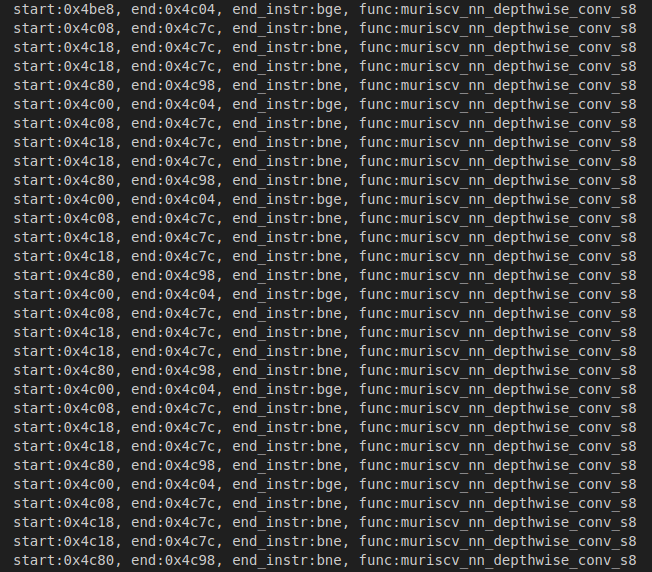
\includegraphics[width=\linewidth]{figures/Basic_Block.png}
    \caption{Example of dynamic basic blocks}
    \label{fig:basic_block}
\end{figure}

\subsection{Callgrind Inclusive Cost Collector}
\label{subsec:inclusive_cost}

Inclusive cost includes, taking instruction counts event for example, instructions executed by every child node of the given caller function in the call graph. It is an important source of information to represent caller-callee relations quantitatively.

\medskip

There are three data structures used for inclusive cost collection:

\begin{itemize}
    \item Call stack: It stores the name of each function in caller-callee relation.
    \item Basic block stack: It stores \texttt{BasicBlock} instances of each function. In other words, it is a list of lists in python. 
    \item Inclusive cost dictionary: it stores the mapping between the program counter of branch instruction and the program counter it jumps to together with the corresponding cost. 
\end{itemize}

As shown in \ref{alg:inclusive_cost_collector}, the algorithm iterates over dynamic basic block list mentioned in section \ref{subsec:bb_construction}. It deals with three cases:

\begin{itemize}
    \item Calling another function: Call stack appends the function name of current basic block and basic block stack appends current basic block instance as a python list.
    \item Jumping inside the same function: The last element in basic block stack appends current basic block instance.
    \item Returning from callee: First, the distance between callee function and the function it returns to is calculated. Afterwards, the cost is accumulated throughout each caller-callee relation. Taking the example shown in fig\ref{fig:analyzer_inclusive_cost}, \texttt{Function B} returns to \texttt{Function A}. Instruction counts for each dynamic basic block in \texttt{Function B} are added up, which are available inside each \texttt{BasicBlock} instance. Besides, subroutine cost of \texttt{bb3}, which means all the instruction counts of its subgraph and is annotated between parentheses, is also added up. The accumulation is simply \texttt{56+8+24+16=104} and the resulting number becomes subroutine cost of \texttt{bb1}. At the very end, this iterative procedure yields inclusive cost dictionary and finally prepare us for generating callgrind output format file. 
\end{itemize}

\medskip
\begin{algorithm}
\caption{Callgrind Inclusive Cost Collector}
\label{alg:inclusive_cost_collector}
\begin{algorithmic}
\REQUIRE $dynamic\_basic\_blocks\_list$
\STATE $call\_stack \gets\ []$
\STATE $bb\_stack \gets\ []$
\STATE $inclusive\_cost\_dictionary \gets\ \{\}$
\STATE $previous\_bb \gets\ None$
\FOR{$current\_bb$ in $dynamic\_basic\_block\_list$}
    \IF{$previous\_bb = None$ or ($previous\_bb.last\_instruction$ is branch instruction and $current\_bb.function \neq prev\_bb.function$)}
        \STATE $call\_stack$.append($current\_bb.function$)
        \STATE $bb\_stack$.append([$current\_bb$])
    \ELSIF{$current\_bb.function = prev\_bb.function$}
        \STATE $bb\_stack$[-1].append($current\_bb$)
    \ELSIF{$previous\_bb.last\_instruction = jalr$}
        \STATE calculate $distance$ between $previous\_bb$ and $current\_bb$
        \FOR{$i$ in range($distance$)}
            \STATE accumulate instruction counts and subroutine cost
        \ENDFOR
    \ENDIF
    \STATE $current\_bb \gets\ previous\_bb$
\ENDFOR
\end{algorithmic}
\end{algorithm}
\medskip

\begin{figure}
    \centering
    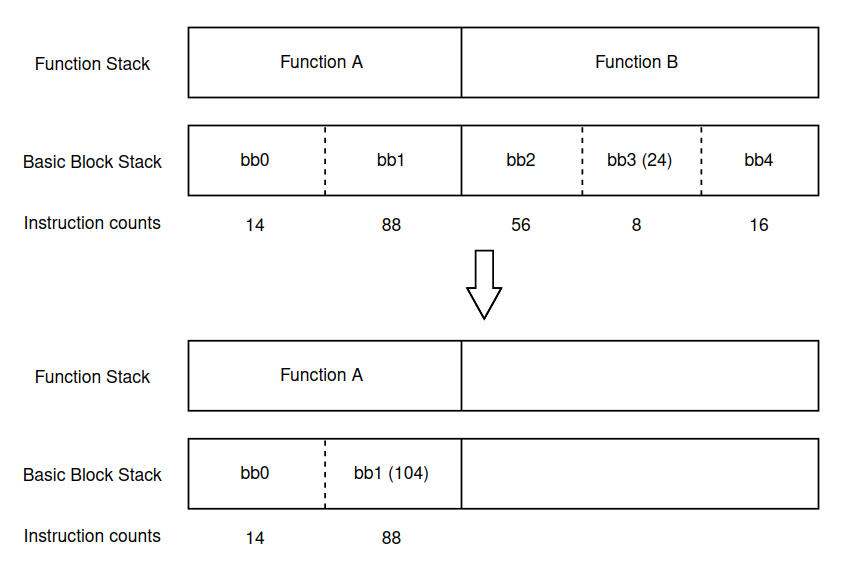
\includegraphics[width=\linewidth]{figures/Analyzer_inclusive_cost.png}
    \caption{Illustration of inclusive cost collection}
    \label{fig:analyzer_inclusive_cost}
\end{figure}
                    
\subsection{Callgrind Output Format Converter}
\label{subsec:converter}

Generating callgrind output format file is the last step. The format serves as the common language between callgrind and GUI tool kcachegrind. The full specification won't be discussed here in detail; instead, only the basic structure and the specification for representing caller-callee relations are important for the scope of this work, which are shown in listing \ref{code:callgrind_output_format}. First of all, the header should contain magic words \texttt{\# callgrind format}. It should also specify positions and events information. In our case, they are \texttt{positions: instr} and \texttt{events: Instructions}. Regarding general structure, for each function, all of its positions and corresponding cost information are printed in ascending order. As for caller-callee relations, taking the example in fig \ref{fig:callgrind_output_format}, the instruction at address \texttt{0x56c} jumps to address \texttt{0x608} for once (\texttt{calls=1}), which belongs to function \texttt{TVMWrap\_GetInputPtr}. And the inclusive cost of \texttt{0x56c} is 6 (\texttt{0x56c 6}).

\lstset{
  basicstyle=\footnotesize\ttfamily,
  breaklines=true,
  frame=single,
  showstringspaces=false,
  captionpos=b
}

\begin{center}
\begin{minipage}{\textwidth}
\lstset{caption={Callgrind output format}, label=code:callgrind_output_format}
\begin{lstlisting}
## header
# callgrind format
version:
creator:
pid:
cmd:

positions: (types of position, e.g. instr and pos)
events: (types of events, e.g. Instructions, Cycles, Flops, and ticks)

## general structure
ob=(ELF file)
fl=(source file)
fn=(function)
(positions) (cost)
...

## example of caller-callee relation
(positions) (cost)
cob=(ELF file of callee)
cfi=(source file of callee)
cfn=(callee function)
calls=(number of calls) (target position)
(positions) (inclusive cost)
\end{lstlisting}
\end{minipage}
\end{center}

\begin{figure}
    \centering
    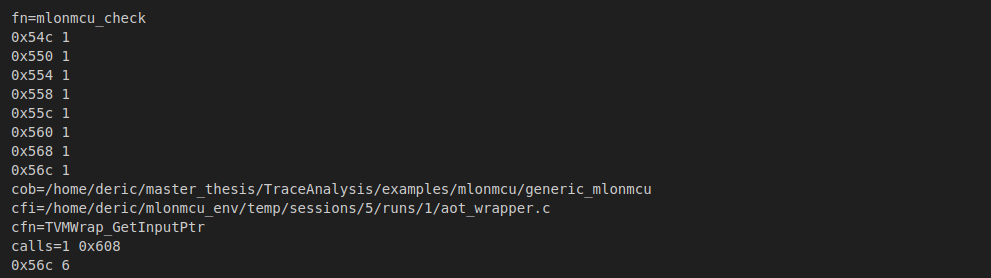
\includegraphics[width=\linewidth]{figures/Output_format_example.png}
    \caption{Example of callgrind output format}
    \label{fig:callgrind_output_format}
\end{figure}

\section{Optimization}
As the workflow and implementation details are shown in previous sections, the question to be asked is - Can we do better? Regarding memory usage of \texttt{BasicBlock} instances and time complexity of the query utility functions, there is indeed room for optimization. 

\subsection{\texttt{BasicBlock} class}
\label{subsec:basicblock_optimization}

Recall from section \ref{subsec:bb_construction} that new \texttt{BasicBlock} instances are contructed over and over again during iterating through instruction trace. However, instances having same values of variables \texttt{start\_pc}, \texttt{last\_pc}, \texttt{last\_instr}, and \texttt{func} should not coexist since they represent same semantics. In fact, for application program that contains many loop structures, especially machine learning applications, original implementation of \texttt{BasicBlock} object wastes too much memory or might even drain RAM space.

Flyweight design pattern comes into play for solving the issue. A common approach is implementing \texttt{BasicBlockFactory} class besides to \texttt{BasicBlock} class. The factory class serves as an interface between client application and original \texttt{BasicBlock} class. It maintains an internal data structure and responds properly to requests. A instance is created only when it doesn't exist in internal data structure.

There is also a more python-oriented approach. In python, \texttt{\_\_new\_\_} and \texttt{\_\_init\_\_} are two important methods for creation and initialization of objects. Static method \texttt{\_\_new\_\_} is called before instance method \texttt{\_\_init\_\_}. As shown in Listing \ref{code:BasicBlock_class}, we can control the process of instance creation in \texttt{\_\_new\_\_}. Namely, an internal data structure \texttt{\_instances} stores the mapping between self-defined key and instance. If the instance exists, \texttt{\_\_new\_\_} directly returns it; otherwise, \texttt{\_\_new\_\_} creates one and returns it.

Table \ref{tab:comparison_mem_usage} quantifies the comparison between original implementation and optimization using flyweight design pattern regarding number of \texttt{BasicBlock} instances and their memory usage. Python library \texttt{pymler} is used for inspecting memory usage. It turns that both are reduced by more than 99\% on all four ML models. For smaller models, such as \textit{toycar} and \textit{aww}, this optimization is a nice-to-have. And it becomes a must for larger models such as \texttt{vww} and \texttt{resnet}.

\medskip
\begin{table}[h!]
    \centering
    \resizebox{\textwidth}{!}{
    \begin{tabular}{|c|c|c|c|c|}
    \hline
    \multirow{2}{*}{model}  & \multicolumn{2}{|c|}{original implementation} & \multicolumn{2}{|c|}{with flyweight design pattern} \\
    \cline{2-5}
     & \texttt{BasicBlock} instances & memory usage & \texttt{BasicBlock} instances & memory usage \\
    \hline
     toycar & 99772 & 53.2 MB & 394 & 408 KB \\ 
    \hline
     aww    & 869587 & 564 MB & 669 & 803 KB \\
    \hline
     vww    & 2685142 & 1.4 GB & 765 & 935 KB \\
    \hline
     resnet & 2709481 & 1.41 GB & 617 & 742 KB \\
    \hline
    \end{tabular}
    }
    \caption{Comparison of total memory usage of \texttt{BasicBlock} instances}
    \label{tab:comparison_mem_usage}
\end{table}

\medskip
\begin{center}
\begin{minipage}{\textwidth}
\lstset{caption={BasicBlock class}, label=code:BasicBlock_class}
\begin{lstlisting}
class BasicBlock(object):
    _instances = {}

    def __new__(cls, first_pc: int, last_pc: int, last_instr: str, func: str):
        key = (first_pc, last_pc, last_instr, func)
        instance = cls._instance.get(key)
        if instance is None:
            instance = super().__new__(cls)
            cls._instance[key] = instance
            instance.__initialized = False
            instance._freq = 0
        instance._freq += 1
        return instance

    def __init__(self, first_pc: int, last_pc: int, last_instr: str, func: str):
        if not self.__initialized:
            self.first_pc = first_pc
            self.last_pc = last_pc
            self.func = func
            self.last_instr = last_instr
            self.__initialized = True

\end{lstlisting}
\end{minipage}
\end{center}


\subsection{Query}
Recall from section \ref{subsec:elf_info_extraction}, there are two utility functions based on program counter to function name mapping and program counter to source line mapping respectively. Given that they are extensively used during dynamic basicblocks construction and callgrind output format conversion, their performance matters. Naively, taking function name query function for example, each key-value pair in \texttt{pc\_to\_func\_mapping} is iterated through in order to find out \texttt{func\_name}, as shown in listing \ref{code:naive_implementation}. The time complexity turns out to be O(n). To improve it, binary search comes into play. First of all,\texttt{pc\_to\_func\_mapping} is no longer a python \texttt{dict}; instead, it is a python \texttt{list} that stores \texttt{(start\_pc, end\_pc, func\_name)} as tuple. And it is sorted in ascending order based on \texttt{start\_pc}. Then we use python \texttt{bisect} library to do binary search, as shown in listing \ref{code:binary_search_func_name}. 

\medskip
\begin{center}
\begin{minipage}{\textwidth}
\lstset{caption={Naive Implementation}, label=code:naive_implementation}
\begin{lstlisting}
# Assume pc_to_func_mapping is given
# pc_to_func_mapping: {func_name : (start_pc, end_pc)}

def find_func_name(pc: int) -> str:
    for func_name, range in pc_to_func_mapping.items():
        if range[0] <= pc <= range[1]:
            return func_name
    return "???"

\end{lstlisting}
\end{minipage}
\end{center}

\begin{center}
\begin{minipage}{\textwidth}
\lstset{caption={Using binary search}, label=code:binary_search_func_name}
\begin{lstlisting}
import bisect

# pc_to_func_mapping is now a list and
# is sorted in ascending order based on start_pc
# pc_to_func_mapping: (start_pc, end_pc, func_name) 
# pc_to_func_mapping.sort(key=lambda x : x[0])

def find_func_name(pc: int) -> str:
    i = bisect.bisect_right(pc_to_func_mapping, pc, key=lambda x : x[0])
    if i > 0:
        start_pc, end_pc, func_name = pc_to_fun_mapping[i-1]
        if start_pc <= pc <= end_pc:
            return func_name
    return "???"
    
\end{lstlisting}
\end{minipage}
\end{center}

Similarly, 

\begin{center}
\begin{minipage}{\textwidth}
\lstset{caption={Using binary search}, label=code:binary_search_source_line}
\begin{lstlisting}
import bisect

# Asssume pc_to_source_line_mapping is given
# pc_to_source_line_mapping : {source_file : [(pc, source_line), ...]}

def dump_source_line(pc: int, source_file: str) -> str:
    if source_file == "???":
        return "0"
    mapping = pc_to_source_line_mapping[source_file]
    i = bisect.bisect_right(mapping, pc, key=lambda x : x[0])
    if i > 0:
        start_pc, line = mapping[i-1]
        if pc >= start_pc:
            return f"{line}"
    return "0"

\end{lstlisting}
\end{minipage}
\end{center}